\documentclass[journal]{IEEEtran}

% Common packages (template)
\usepackage{graphicx}
\usepackage{amsmath}
\usepackage{amssymb}
\usepackage{hyperref}
\usepackage{float}
\usepackage{subcaption}
\usepackage{booktabs}
\usepackage{pgfplotstable}
\usepackage{siunitx}
\usepackage{qrcode}

\pgfplotsset{compat=1.18}

\pgfplotstableset{
	col sep=comma,
	every head row/.style={before row=\toprule, after row=\midrule},
	every last row/.style={after row=\bottomrule},
}

\begin{document}

% ---------- TITLE & AUTHOR ----------
\title{Equation of State for an Ideal Gas}
\author{IBRAHIM H.I. ABUSHAWISH \\
Istanbul University, Department of Physics \\
Instructor: Res. Asst. PhD ERDİNÇ ULAŞ SAKA \\
Experiment Date: 02.03.2026 , Report Submission Date: \\
Course \& Section Number: PHYS3604}

\markboth{Physics Laboratory Reports, March 2026}{}

\maketitle

% ---------- ABSTRACT ----------
\begin{abstract}
The ideal gas law was investigated through three processes for a fixed amount of gas: isothermal compression/expansion (Boyle--Mariotte), isobaric heating (Gay--Lussac/Charles), and isochoric heating (Amontons). From manometer and geometric volume readings, the universal gas constant was calculated as $\bar{R}=\SI{8.188}{\joule\per\mole\per\kelvin}$ with a sample standard deviation $s_R=\SI{0.0343}{\joule\per\mole\per\kelvin}$ (relative deviation $\approx\SI{0.42}{\percent}$) and a percent error of $\SI{-1.53}{\percent}$ relative to $R_\mathrm{ref}=\SI{8.314}{\joule\per\mole\per\kelvin}$. Linear regressions confirmed $V\propto T$ at constant pressure and $P\propto T$ at constant volume with $R^2\approx 1$.
\end{abstract}

% ---------- INTRODUCTION ----------
\section{Introduction}
The macroscopic state of a gas is characterized by pressure $p$, volume $V$, temperature $T$, and amount of substance $n$. In the ideal-gas limit (low density), these variables are related by the ideal gas equation of state. The purpose of this experiment is (i) to test the validity of the three classical gas laws for a constant quantity of gas under controlled conditions and (ii) to determine the universal gas constant $R$ as well as the thermal expansion and thermal stress coefficients from the measured relationships \cite{lab_manual}.

% ---------- THEORY ----------
\section{Theory}
For an ideal gas,
\begin{equation}
	pV = nRT.
	\label{eq:ideal_gas}
\end{equation}

\subsection{Boyle--Mariotte (Isothermal)}
At constant temperature ($T=\mathrm{const.}$) and fixed $n$, Eq.~\eqref{eq:ideal_gas} gives
\begin{equation}
	pV = \mathrm{const.}\quad\Rightarrow\quad p \propto \frac{1}{V}.
	\label{eq:boyle}
\end{equation}

\subsection{Gay--Lussac/Charles (Isobaric)}
At constant pressure ($p=\mathrm{const.}$) and fixed $n$,
\begin{equation}
	\frac{V}{T} = \mathrm{const.}\quad\Rightarrow\quad V \propto T.
	\label{eq:charles}
\end{equation}

\subsection{Amontons (Isochoric)}
At constant volume ($V=\mathrm{const.}$) and fixed $n$,
\begin{equation}
	\frac{p}{T} = \mathrm{const.}\quad\Rightarrow\quad p \propto T.
	\label{eq:amontons}
\end{equation}

\subsection{\texorpdfstring{Coefficients $\gamma_0$ and $\beta_0$}{Coefficients gamma0 and beta0}}
Following the lab manual, the slopes of the isobaric and isochoric linear relationships can be expressed as \cite{lab_manual}
\begin{equation}
	\left(\frac{\partial V}{\partial T}\right)_{p,n} = V_0\gamma_0,
	\label{eq:gamma_def}
\end{equation}
\begin{equation}
	\left(\frac{\partial p}{\partial T}\right)_{V,n} = p_0\beta_0,
	\label{eq:beta_def}
\end{equation}
where $V_0$ and $p_0$ are the extrapolated values at $T_0=\SI{273.15}{\kelvin}$. With linear fits $V=aT+b$ and $p=cT+d$, one obtains
\begin{equation}
	\gamma_0 = \frac{a}{V(T_0)},\qquad \beta_0 = \frac{c}{p(T_0)}.
	\label{eq:gamma_beta_from_fit}
\end{equation}

% ---------- EXPERIMENTAL SETUP ----------
\section{Experimental Setup}
The experiment uses a gas-law apparatus with a graduated measuring tube and mercury manometer, immersed in a thermostated water bath. The main equipment listed in the manual includes the gas law unit, circulating thermostat (bath), and thermometer \cite{lab_manual}. The pressure difference is read from the mercury height difference $\Delta h$, while the gas volume is inferred from the measured air-column length $L$ and the tube geometry.

% ---------- PROCEDURE ----------
\section{Experimental Procedure}
The procedure is summarized directly from the lab manual \cite{lab_manual}.

\subsection{Part I: Isothermal (Boyle--Mariotte)}
\begin{enumerate}
	\item Fill the thermostat bath with water.
	\item Set the thermostat to \SI{30}{\celsius} and wait for stabilization.
	\item By moving the gas laws unit, examine the pressure--volume relationship at constant temperature and record it in Table~\ref{tab:table1}.
	\item Draw the $p$--$V$ graph and compute $R$ for each measurement.
\end{enumerate}

\subsection{Part II: Isobaric (Gay--Lussac/Charles)}
\begin{enumerate}
	\item At \SI{30}{\celsius}, equalize the mercury columns ($\Delta h=0$). Measure $L_0$, compute $V_0$, and record the reference values.
	\item Raise the temperature to \SI{40}{\celsius}. With $\Delta h=0$, measure $L$ and compute $V$, and record in Table~\ref{tab:table2}.
	\item Repeat in \SI{10}{\celsius} steps up to \SI{60}{\celsius}.
\end{enumerate}

\subsection{Part III: Isochoric (Amontons)}
\begin{enumerate}
	\item For each temperature step, bring the mercury level in the measuring tube back to the $L_0$ position.
	\item Read $\Delta h$, compute $p$, and record in Table~\ref{tab:table3}.
\end{enumerate}

% ---------- DATA ANALYSIS ----------
\section{Data Analysis}

\subsection{Assumptions and applied corrections}
In the data reduction, several apparatus-specific constants were required. The atmospheric reference pressure was not measured with a separate barometer during the experiment; instead, the value $p_0=\SI{100.3}{\kilo\pascal}$ provided in the PHYWE apparatus documentation was adopted as the baseline for $\Delta h=0$ \cite{phywe_manual}. In addition, the geometric volume model included a fixed additional volume $V_{\mathrm{add}}=\SI{1.01}{\milli\liter}$, corresponding to the dead volume of the tube section indicated in the apparatus documentation (``brown'' section) \cite{phywe_manual}. The amount of gas was treated as constant and taken as $n=\SI{0.9536}{\milli\mole}$ from the same source \cite{phywe_manual}. These assumptions affect the absolute scale of the calculated quantities (particularly $p$ and $R$) and are therefore stated explicitly here.

\subsection{Pressure from manometer}
With mercury in the manometer, the gas pressure was computed from the height difference $\Delta h$ as
\begin{equation}
	p = p_0 + \rho_{\mathrm{Hg}} g\,\Delta h,
	\label{eq:manometer}
\end{equation}
where $p_0$ is the atmospheric pressure at the reference condition ($\Delta h=0$), $\rho_{\mathrm{Hg}}$ is the mercury density, and $g$ is gravitational acceleration. In the analysis, $p_0=\SI{100.3}{\kilo\pascal}$ was adopted from the PHYWE apparatus documentation \cite{phywe_manual}, and $\rho_{\mathrm{Hg}}=\SI{13595}{\kilogram\per\meter\cubed}$ and $g=\SI{9.81}{\meter\per\second\squared}$ were used.

\subsection{Volume from tube geometry}
The gas volume was determined from the measured air-column length $L$ using a cylindrical model,
\begin{equation}
	V(L) = A L + V_{\mathrm{add}},\qquad A=\pi r^2,
	\label{eq:volume_geom}
\end{equation}
with tube radius $r=\SI{5.7}{\milli\meter}$ (diameter \SI{11.4}{\milli\meter}). An additional dead volume $V_{\mathrm{add}}=\SI{1.01}{\milli\liter}$ was included in the volume model to account for the fixed volume of the apparatus tube section specified in the PHYWE documentation \cite{phywe_manual}.

\subsection{Universal gas constant}
For each isothermal data point (Part I), Eq.~\eqref{eq:ideal_gas} was rearranged to
\begin{equation}
	R = \frac{pV}{nT}.
	\label{eq:R_calc}
\end{equation}
For Part I, the gas temperature was maintained at $T=\SI{303.15}{\kelvin}$ (\SI{30}{\celsius}) and the amount of gas was taken as $n=\SI{0.9536}{\milli\mole}$ as specified in the PHYWE apparatus documentation \cite{phywe_manual}. The resulting $R$ values are given in Table~\ref{tab:table1}. The mean and standard deviation were
\begin{equation}
	\bar{R} = \SI{8.188}{\joule\per\mole\per\kelvin},\qquad s_R=\SI{0.0343}{\joule\per\mole\per\kelvin}.
	\label{eq:R_mean_std}
\end{equation}
Relative to $R_{\mathrm{ref}}=\SI{8.314}{\joule\per\mole\per\kelvin}$, the percent error was $\SI{-1.53}{\percent}$.

\subsection{Regression models}
To verify the laws, linear regressions were performed:
\begin{itemize}
	\item Boyle: $p = a\,(1/V)+b$ (fit over $p$ vs $1/V$).
	\item Charles: $V = aT+b$.
	\item Amontons: $p = aT+b$.
\end{itemize}
The fit parameters and $R^2$ values are reported in Table~\ref{tab:fit_summary}.

\subsection{Thermal expansion/stress coefficients}
From the fitted slopes and extrapolated values at $T_0=\SI{273.15}{\kelvin}$, Eq.~\eqref{eq:gamma_beta_from_fit} yields
\begin{equation}
	\gamma_0 = \SI{3.659e-3}{\per\kelvin},\qquad \beta_0 = \SI{3.651e-3}{\per\kelvin}.
	\label{eq:gamma_beta_values}
\end{equation}
These are close to the ideal-gas expectation $1/T_0 \approx \SI{3.661e-3}{\per\kelvin}$.

% ---------- RESULTS ----------
\section{Results}

\subsection{Processed tables}
Measured and processed data are reported in Tables~\ref{tab:table1}--\ref{tab:fit_summary}. A compact summary of key derived quantities is given in Table~\ref{tab:summary}.

\begin{table}[H]
	\centering
	\caption{Summary of derived quantities.}
	\label{tab:summary}
	\pgfplotstabletypeset[
		columns/quantity/.style={column name={Quantity}, string type, string replace*={_}{\_}},
		columns/value/.style={column name={Value}}
	]{tables/report_summary.csv}
\end{table}

\begin{table}[H]
	\centering
	\caption{Part I (isothermal): processed data and calculated $R$ at $T=\SI{303.15}{\kelvin}$.}
	\label{tab:table1}
	\pgfplotstabletypeset[
		columns/L_cm/.style={column name={$L$ (cm)}},
		columns/Delta_h_cm/.style={column name={$\Delta h$ (cm)}},
		columns/V_ml/.style={column name={$V$ (mL)}},
		columns/p_kPa/.style={column name={$p$ (kPa)}},
		columns/R_J_per_molK/.style={column name={$R$ (J\,mol$^{-1}$\,K$^{-1}$)}}
	]{tables/table1_processed.csv}
\end{table}

\begin{table}[H]
	\centering
	\caption{Part II (isobaric): processed temperature and volume data.}
	\label{tab:table2}
	\pgfplotstabletypeset[
		columns/T_K/.style={column name={$T$ (K)}},
		columns/L_cm/.style={column name={$L$ (cm)}},
		columns/V_ml/.style={column name={$V$ (mL)}}
	]{tables/table2_processed.csv}
\end{table}

\begin{table}[H]
	\centering
	\caption{Part III (isochoric): processed temperature and pressure data.}
	\label{tab:table3}
	\pgfplotstabletypeset[
		columns/T_K/.style={column name={$T$ (K)}},
		columns/Delta_h_cm/.style={column name={$\Delta h$ (cm)}},
		columns/P_kPa/.style={column name={$p$ (kPa)}}
	]{tables/table3_processed.csv}
\end{table}

\begin{table}[H]
	\centering
	\caption{Linear fit summary for the three processes.}
	\label{tab:fit_summary}
	\pgfplotstabletypeset[
		columns/relation/.style={column name={Relation}, string type},
		columns/slope/.style={column name={Slope}},
		columns/intercept/.style={column name={Intercept}},
		columns/R2/.style={column name={$R^2$}}
	]{tables/fit_summary.csv}
\end{table}

\subsection{Graphs}
The required graphs are shown in Figures~\ref{fig:boyle}, \ref{fig:charles}, and \ref{fig:amontons}.

\begin{figure}[H]
	\centering
	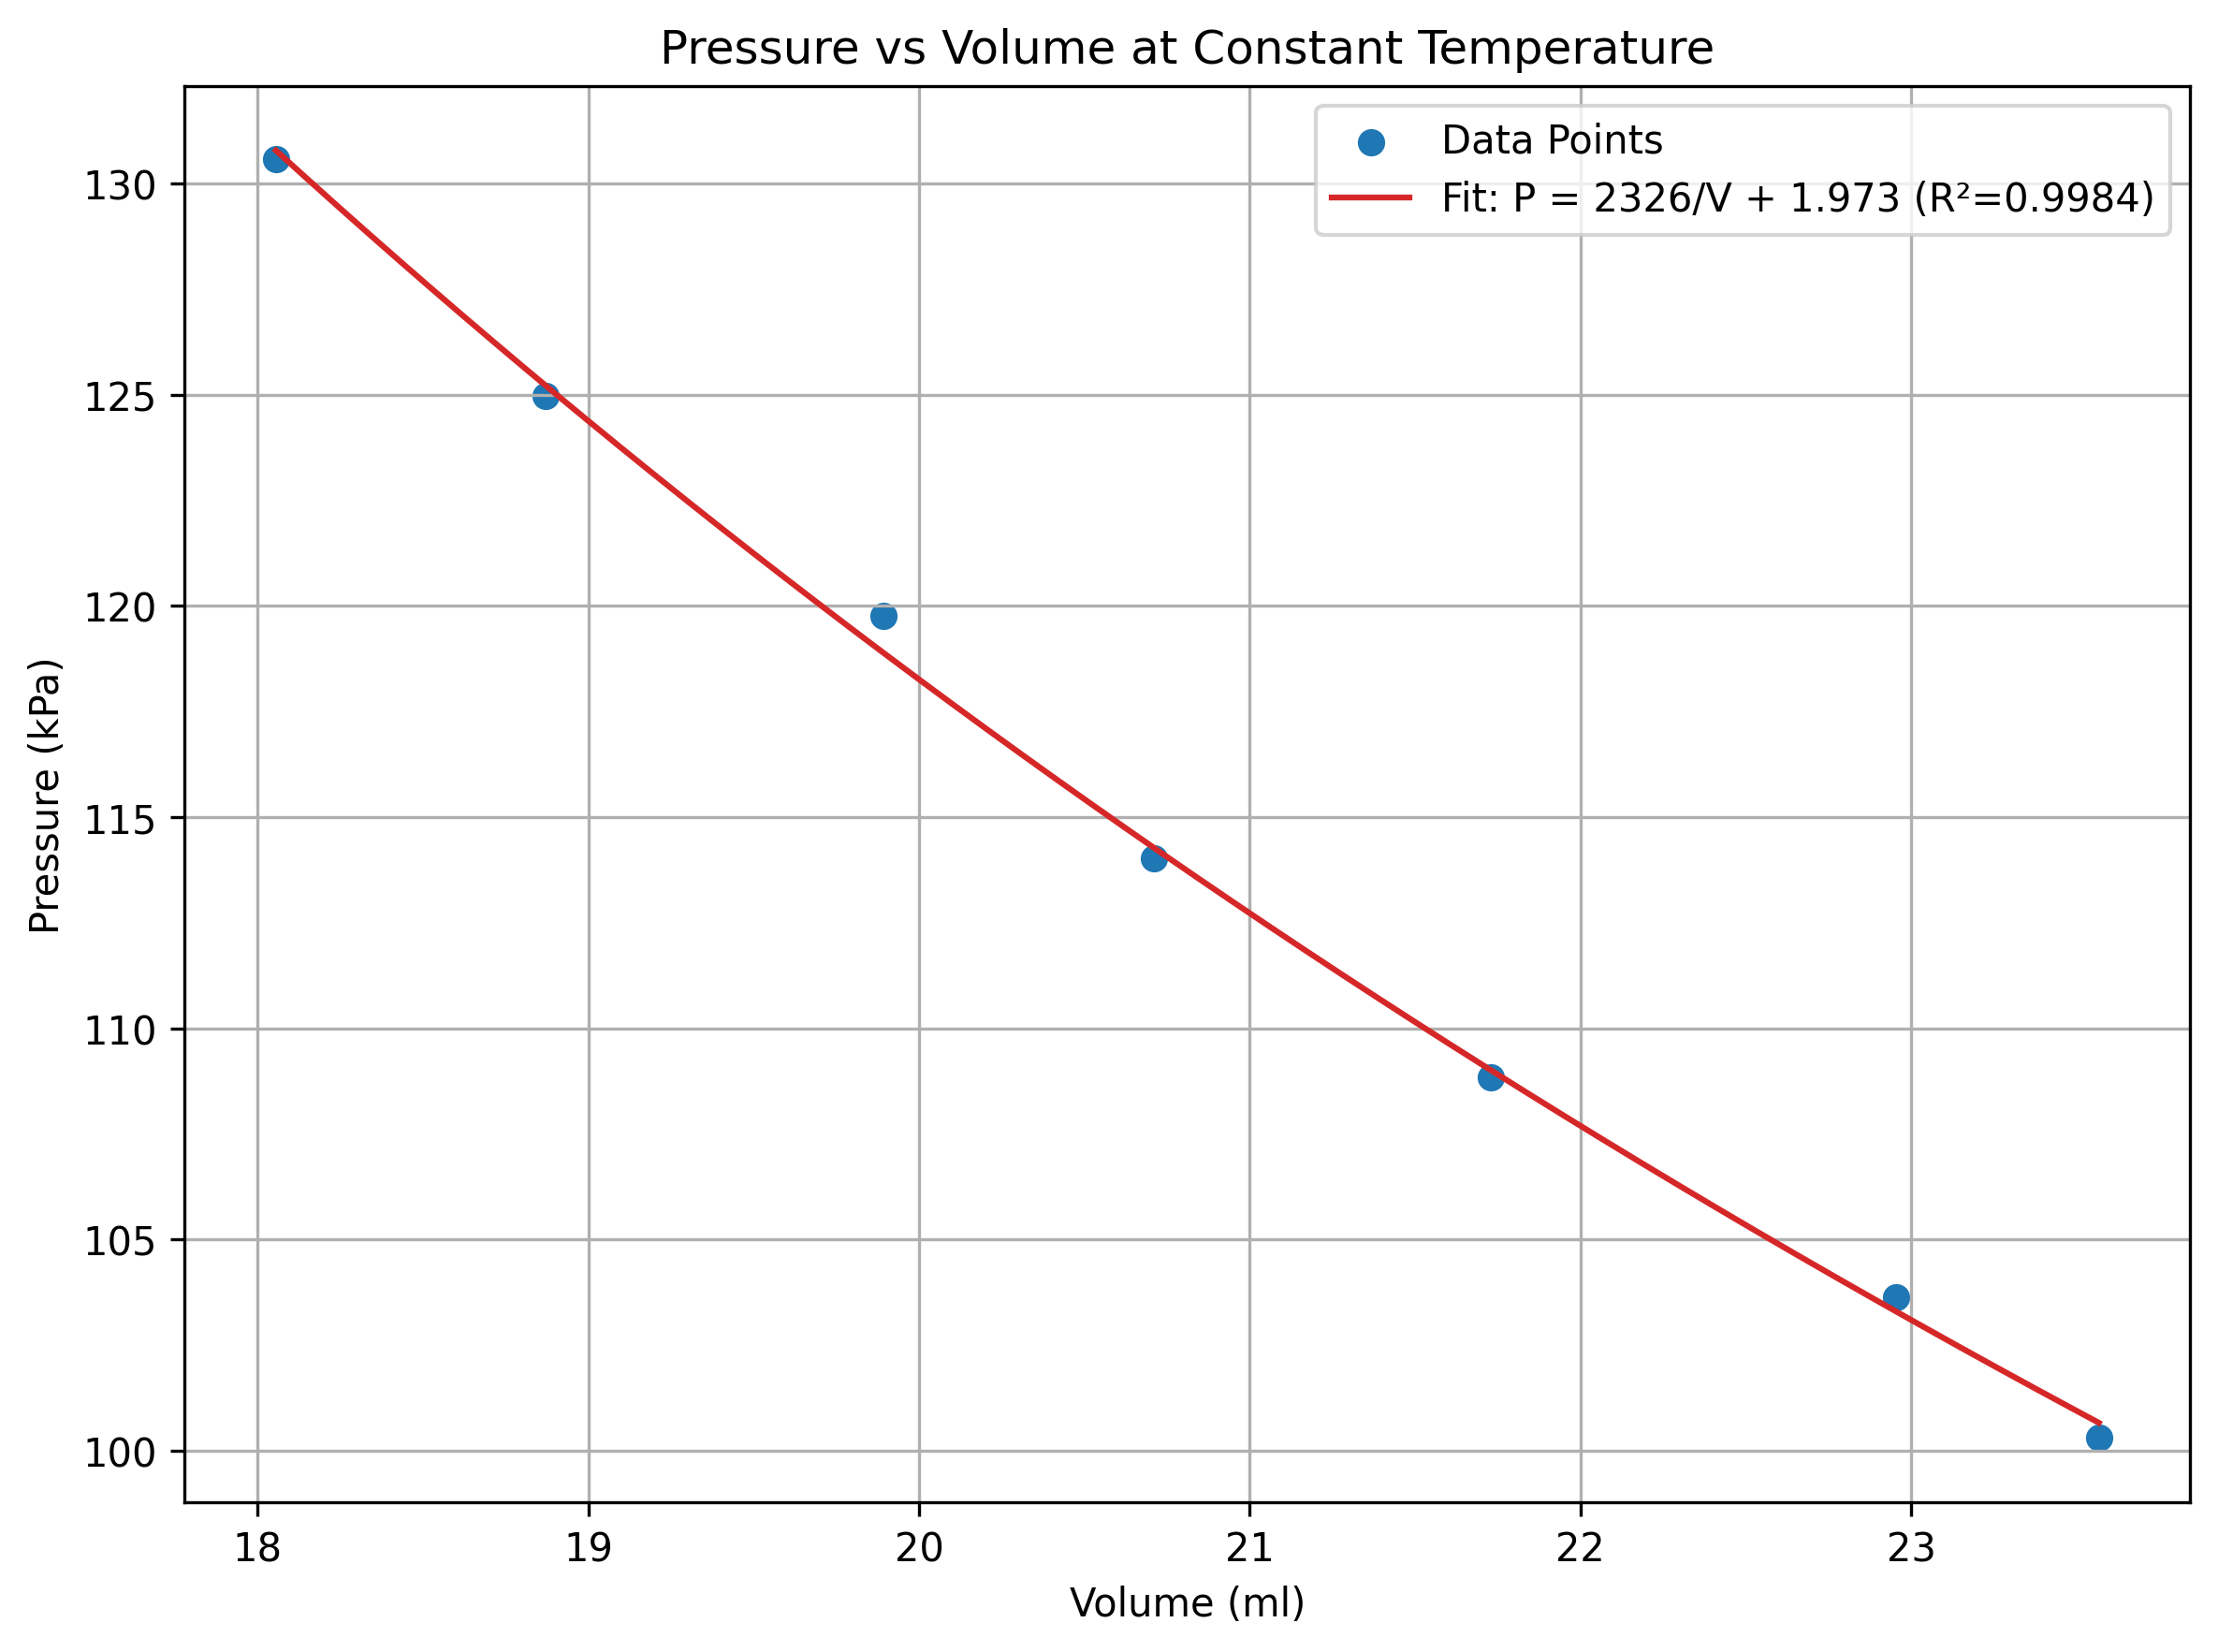
\includegraphics[width=\linewidth]{../plots/boyle_p_vs_v.png}
	\caption{Isothermal data (Part I): pressure versus volume with a $p=a(1/V)+b$ fit.}
	\label{fig:boyle}
\end{figure}

\begin{figure}[H]
	\centering
	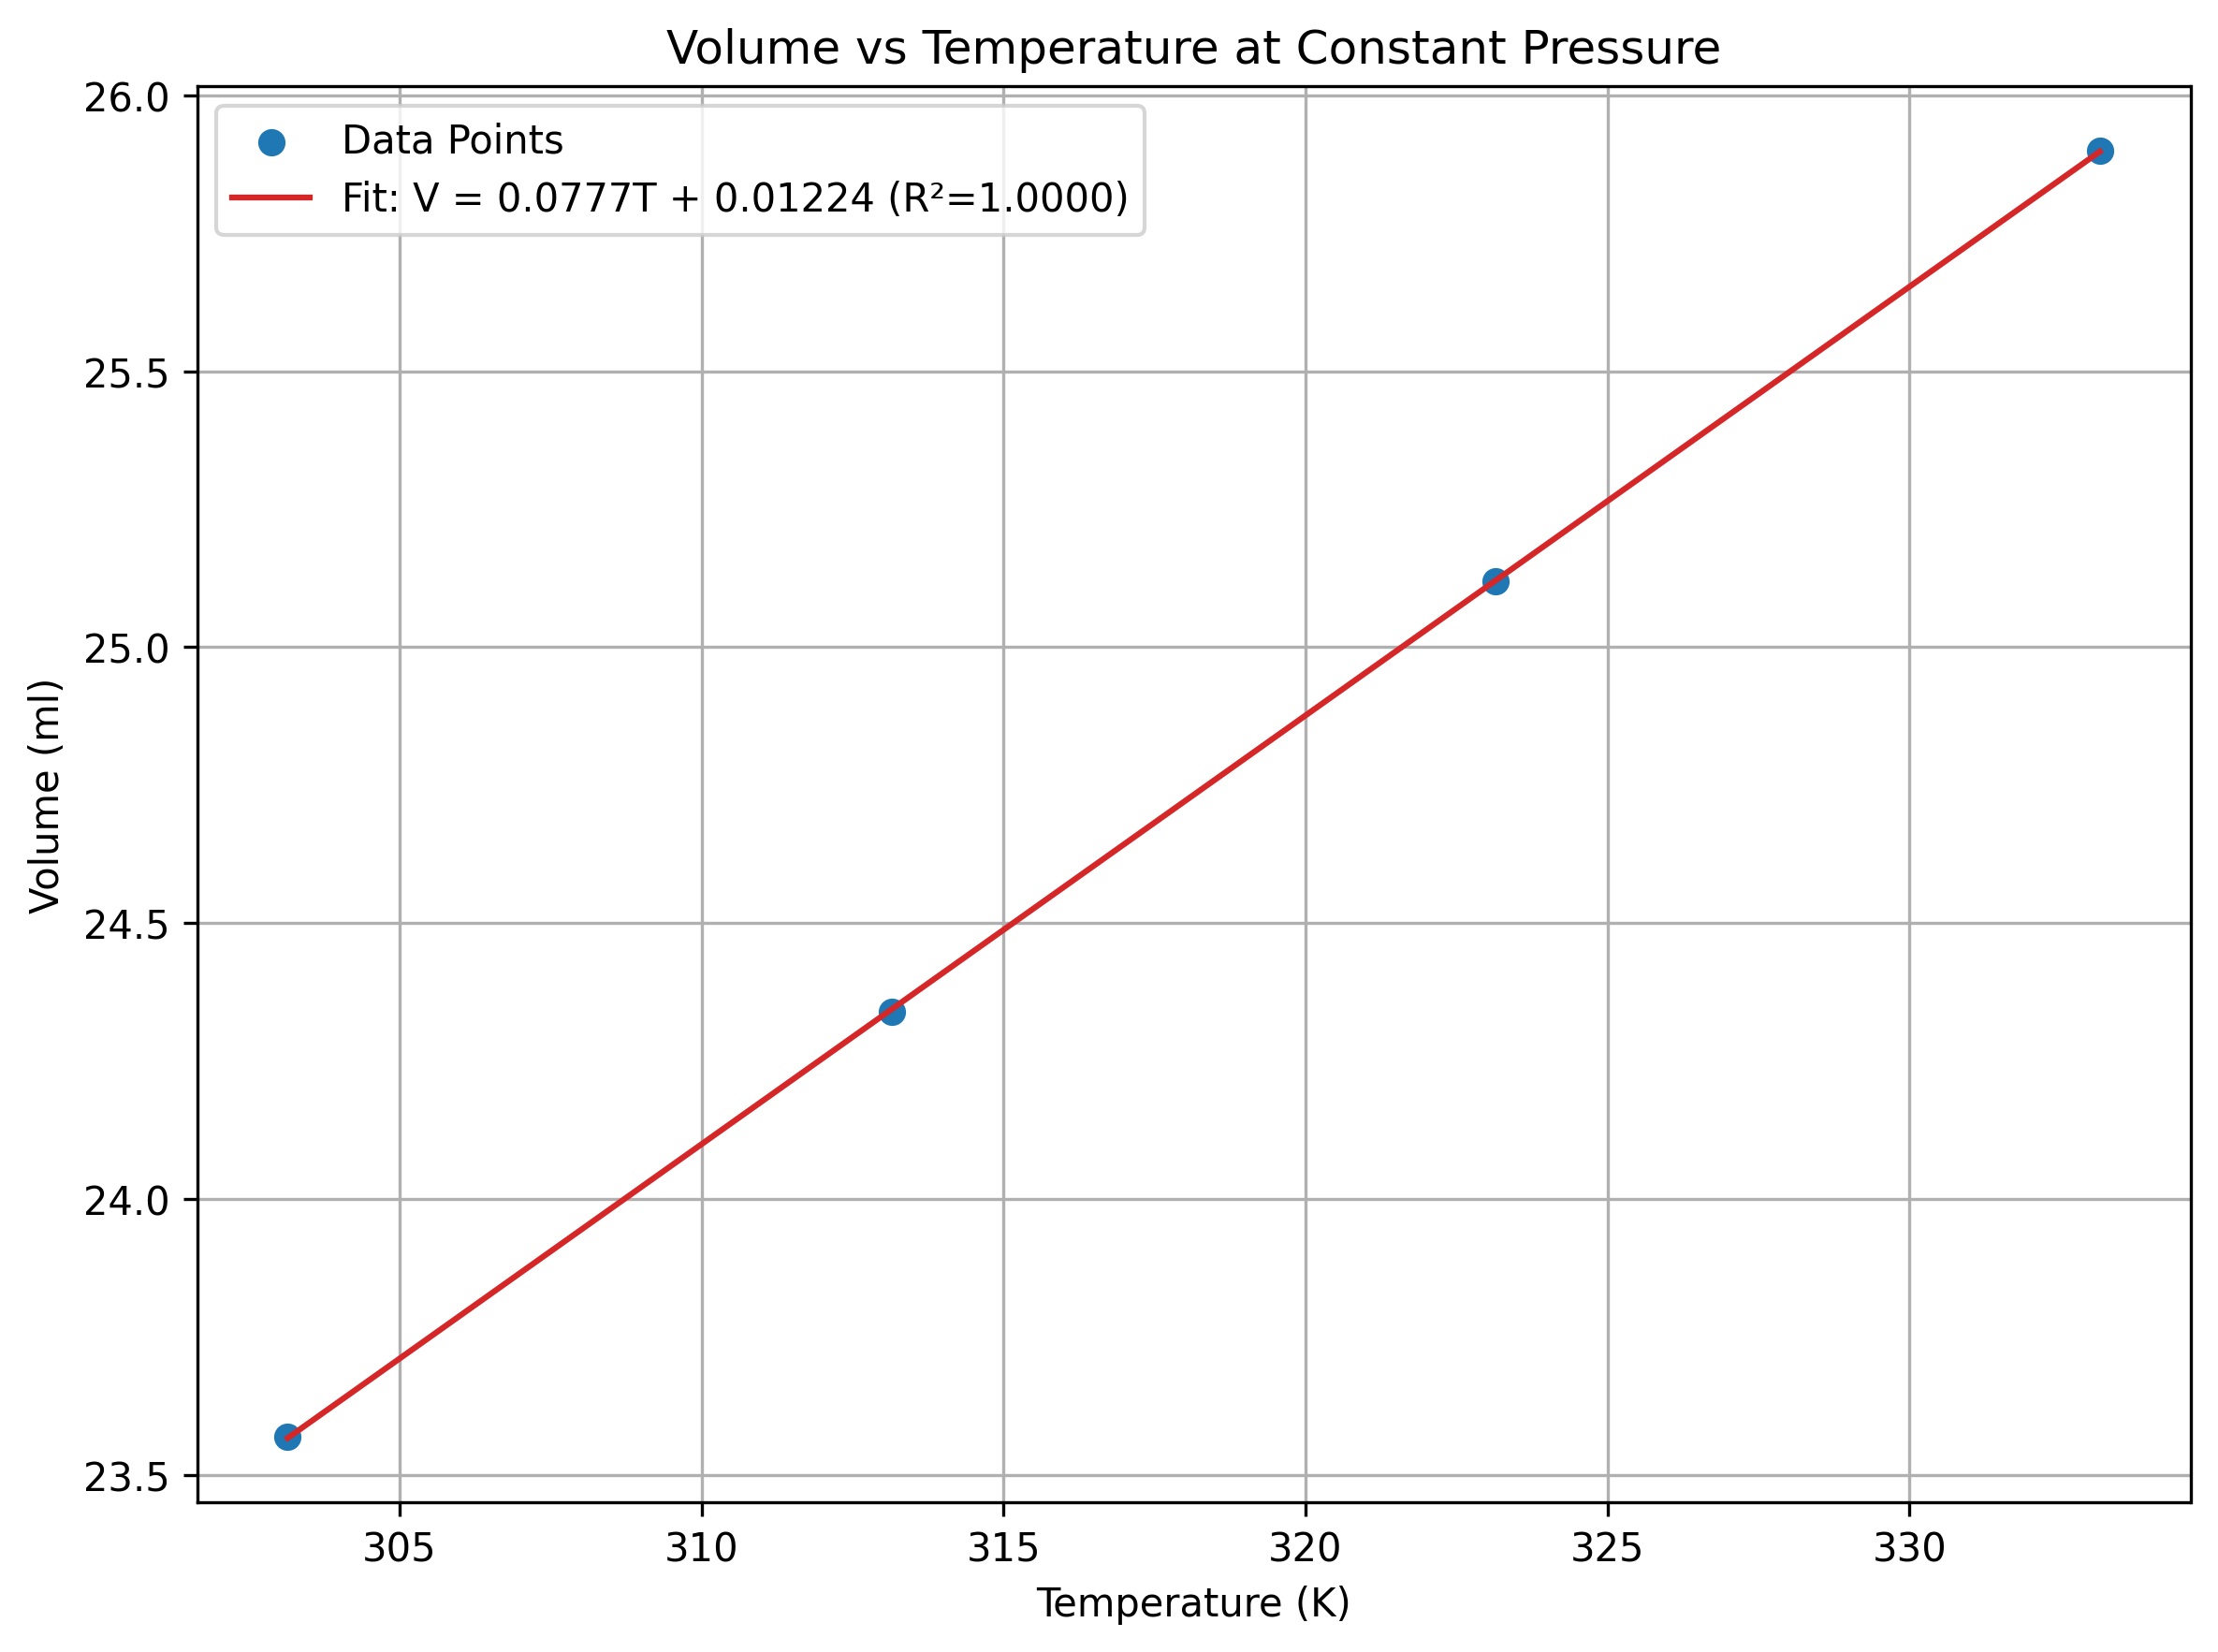
\includegraphics[width=\linewidth]{../plots/charles_v_vs_t.png}
	\caption{Isobaric data (Part II): volume versus temperature with a linear fit.}
	\label{fig:charles}
\end{figure}

\begin{figure}[H]
	\centering
	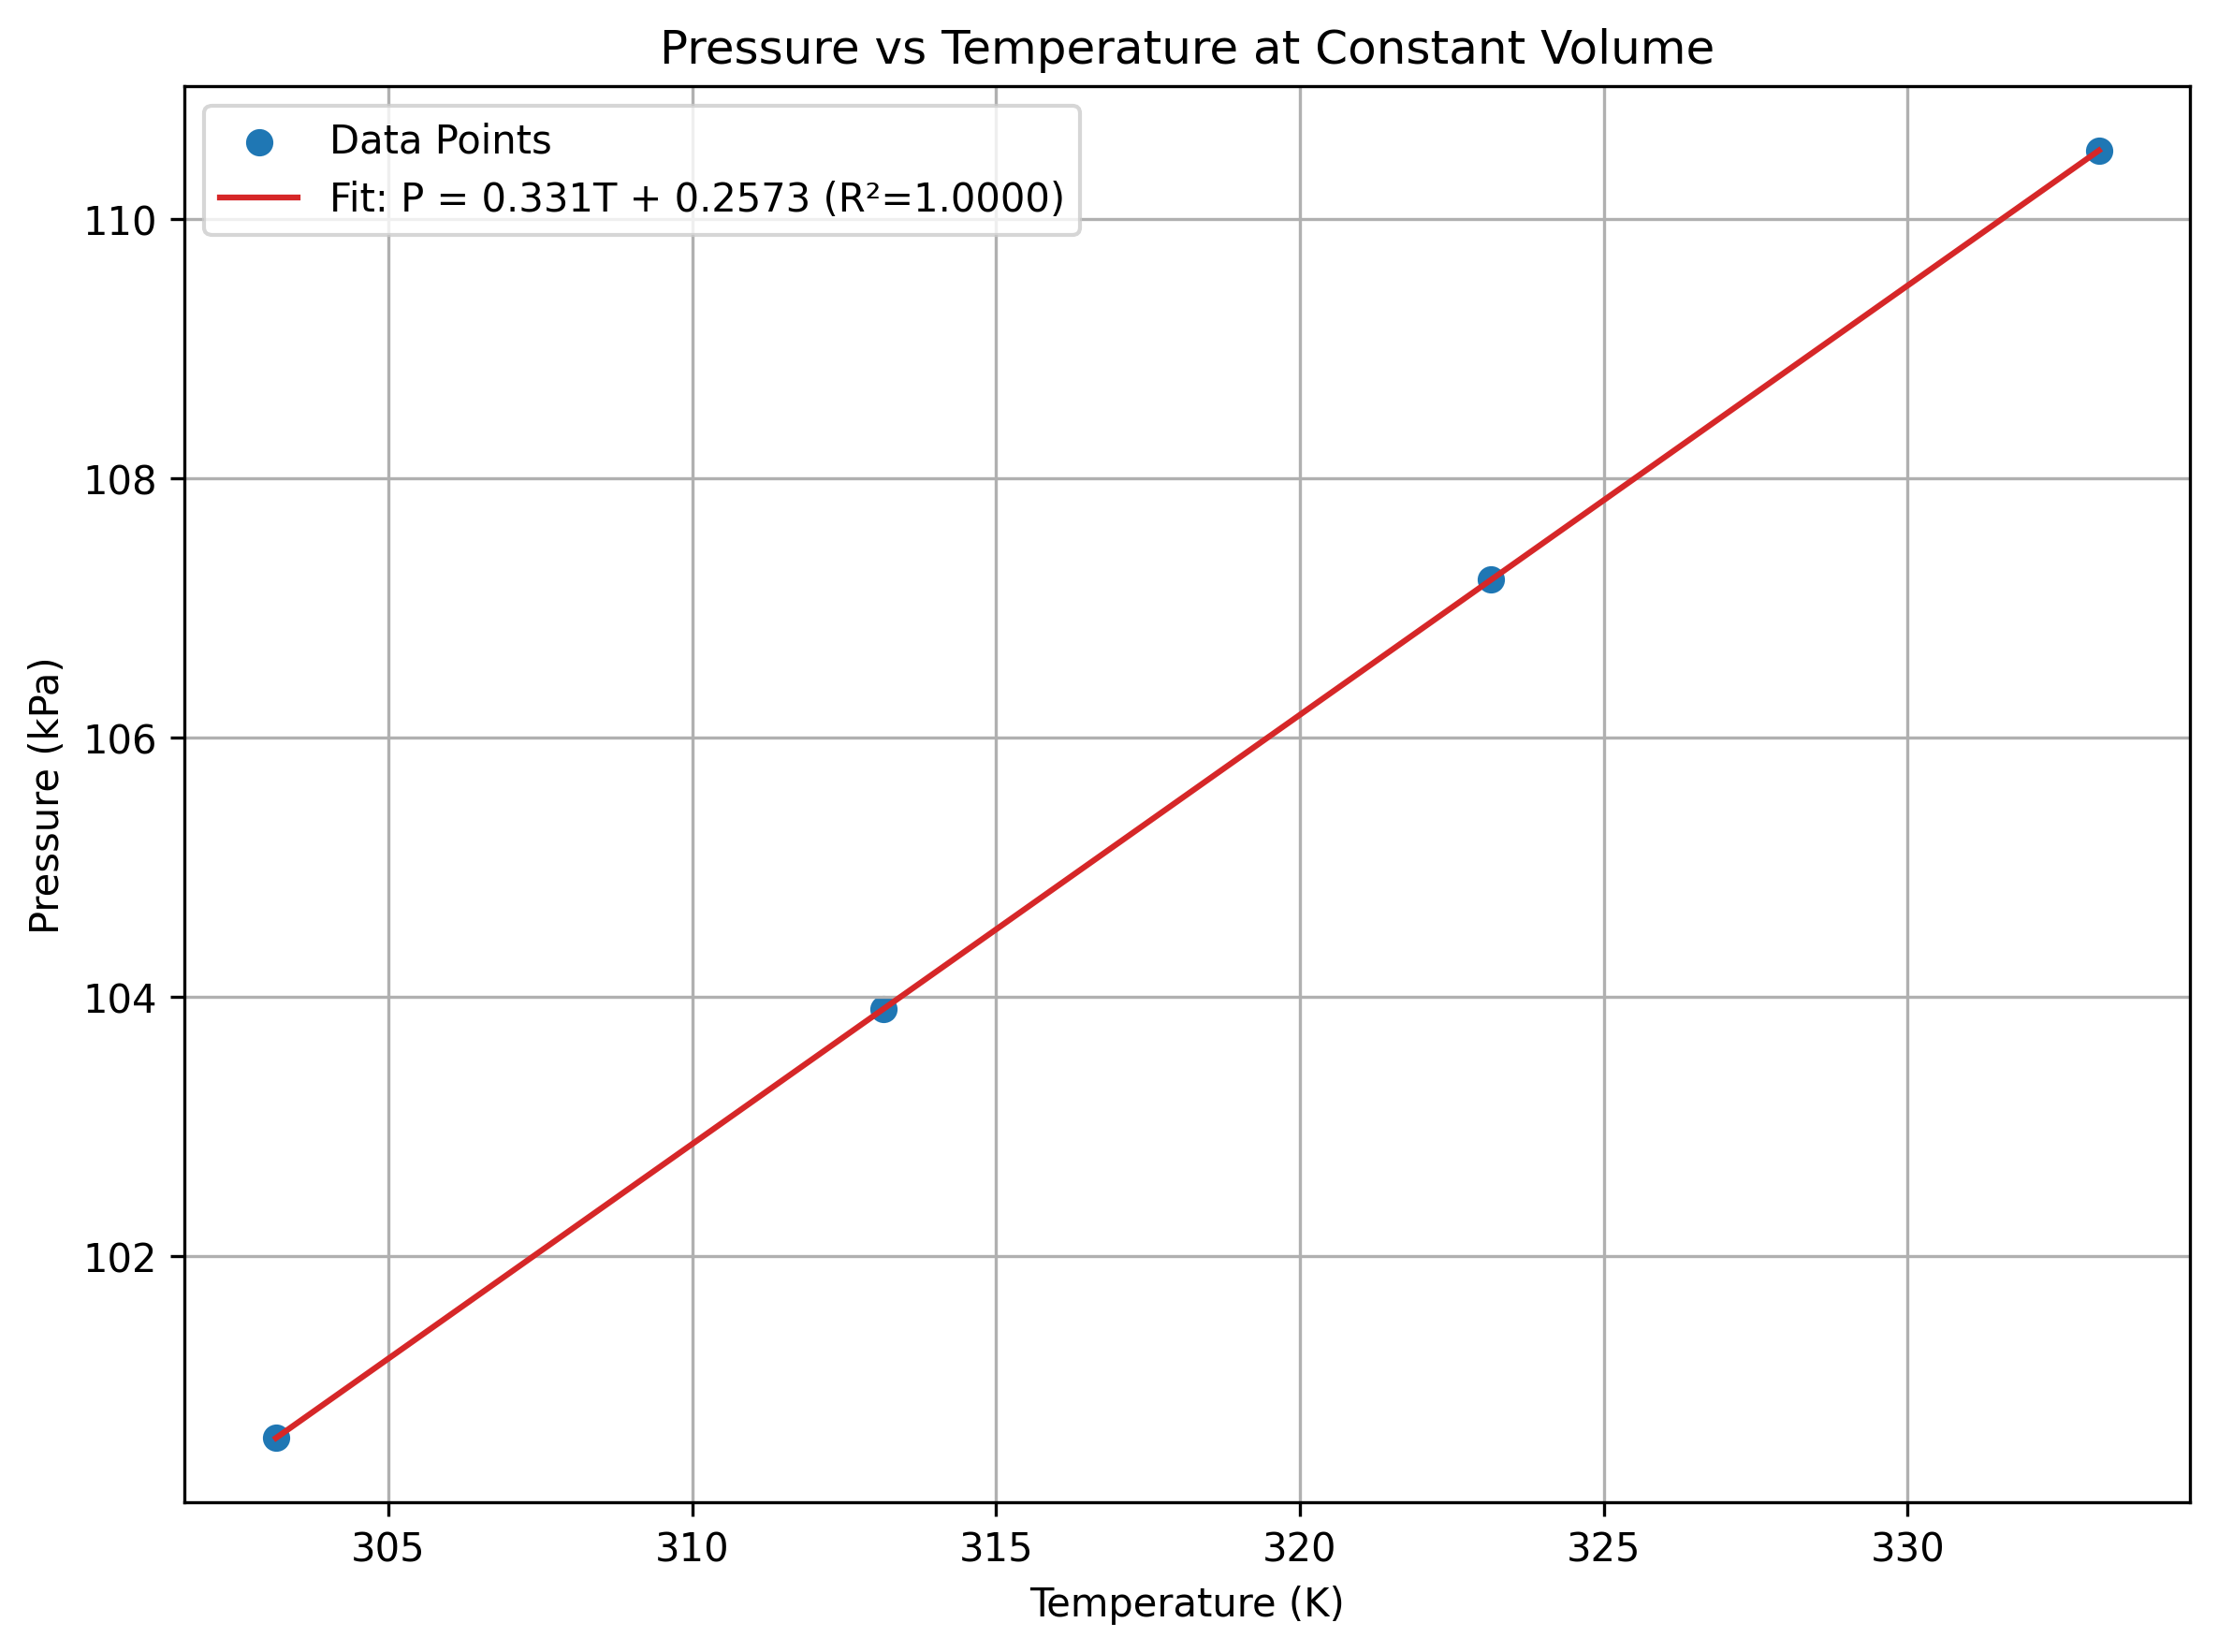
\includegraphics[width=\linewidth]{../plots/amontons_p_vs_t.png}
	\caption{Isochoric data (Part III): pressure versus temperature with a linear fit.}
	\label{fig:amontons}
\end{figure}

% ---------- DISCUSSION ----------
\section{Discussion}
The regression results support the ideal-gas predictions in Eqs.~\eqref{eq:boyle}--\eqref{eq:amontons}. The isobaric and isochoric datasets show excellent linearity ($R^2\approx 1$), consistent with stable temperature control and small experimental scatter.

The gas constant obtained from the isothermal measurements, $\bar{R}=\SI{8.188}{\joule\per\mole\per\kelvin}$, differs from the reference value by about $\SI{-1.53}{\percent}$. Likely contributors are: (i) adopting the reference pressure $p_0=\SI{100.3}{\kilo\pascal}$ from the PHYWE documentation rather than measuring atmospheric pressure during the session, (ii) reading uncertainties in $\Delta h$ (parallax, meniscus) affecting Eq.~\eqref{eq:manometer}, (iii) geometric volume calibration and the apparatus dead-volume correction $V_{\mathrm{add}}=\SI{1.01}{\milli\liter}$ in Eq.~\eqref{eq:volume_geom}, and (iv) small leaks or non-idealities (gas not perfectly ideal, temperature gradients between bath and gas column). Despite these effects, the internal consistency of the computed $R$ across the seven measurements is good (small $s_R$).

The experimentally determined coefficients $\gamma_0$ and $\beta_0$ are close to $1/T_0$ as expected for an ideal gas, which further supports the applicability of the ideal-gas approximation in the explored pressure and temperature ranges.

% ---------- CONCLUSION ----------
\section{Conclusion}
The three classical gas laws were validated for a fixed amount of gas through isothermal, isobaric, and isochoric processes. The universal gas constant was determined as $\bar{R}=\SI{8.188}{\joule\per\mole\per\kelvin}$ with $\SI{-1.53}{\percent}$ error relative to the accepted value. The thermal expansion and thermal stress coefficients were found to be $\gamma_0\approx\SI{3.659e-3}{\per\kelvin}$ and $\beta_0\approx\SI{3.651e-3}{\per\kelvin}$, consistent with the ideal-gas prediction.

% ---------- ADDITIONAL RESOURCES ----------
\section{Additional Resources}
Computational record: \url{https://github.com/ibeuler/LAB-Reports/blob/main/THERMODYNAMICS_AND_STATISTICAL_PHYSICS/1st_Ideal_Gas_Equation/Analysis/calculations.ipynb}.

\begin{figure}[H]
	\centering
	\begin{minipage}{0.15\textwidth}
		\centering
		\qrcode[height=1.5cm]{https://github.com/ibeuler/LAB-Reports}
	\end{minipage}%
	\begin{minipage}{0.2\textwidth}
		\raggedright
		\caption{Access the GitHub repository for source code and related experiments.}
		\label{fig:qr_code}
	\end{minipage}
\end{figure}

\begin{thebibliography}{9}
\bibitem{lab_manual}
	ISTANBUL UNIVERSITY, \textit{Thermodynamics and Statistical Physics Laboratory Experiments Manual}, Department of Physics.

\bibitem{phywe_manual}
	PHYWE Systeme GmbH \& Co. KG, \textit{Laboratory Experiments} (Gas laws apparatus documentation and reference values).
\end{thebibliography}

\end{document}
